\newcommand{\PARAGRAPH}{-20pt}
\newcommand{\ABOVETABLES}{8pt}

\section{LSeq: a polylogarithmic path allocator}
\label{sec:proposal}

\LSEQ (poly\textsc{L}ogarithmic \textsc{SEQ}uence) is the name of the proposed
allocation function.
%Any sequence data structure using
%variable-size identifiers~\cite{preguica2009commutative, weiss2009logoot} can
%use \LSEQ.  
Our prior works~\cite{nedelec2013concurrency, nedelec2013lseq} empirically
showed that \LSEQ allocates identifiers with a sublinear upper bound on space
complexity.  However, we did not provide any complexity analysis to support
these observations.

% \LSEQ improves the space complexity of identifiers by degrading its worst case
% complexity. However, the worst case is made non-trivial. If a malicious user
% tries to produce the worst case scenario, other editors can detect her easily,
% for there is a large difference between the expected space complexity and the
% worst case space complexity.

This section starts by describing the allocation strategy. Then, it provides the
proof of the polylogarithmic growth of \LSEQ's identifiers and states the
conditions upon which this applies. The complexity analysis also includes the
space complexity of a replicated structure, and the time complexity of
operations provided by such structure.

\noindent As for the communication complexity, the next section describes
an \LSEQ-based editor that benefits from these identifiers.

\subsection{Allocation of paths}
\label{subsec:lseqallocation}

When a user types a character, the editor executes the local part of the
\textsc{insert} operation (see Line~\ref{line:insert} of
Algorithm~\ref{algo:crdtabstract}). This function allocates an identifier
comprising a path, the element, and a disambiguator. The most important choice
concerns the path (see Line~\ref{line:allocpath} of
Algorithm~\ref{algo:crdtabstract}).
\noindent The function \textsc{allocPath} chooses the path that encodes the
position of the new element regarding its adjacent elements in the sequence
using a dense space. For the sake of performance, it aims to keep the paths
small.

% General idea is coming... (as winter...)
% \noindent The general idea behind \LSEQ is that it agrees to be temporarily
% inefficient in order to reach a state where it will be efficient enough to
% compensate its past temporary inefficiency.

\begin{algorithm}

\begin{algorithm}[h]
\small
\algrenewcommand{\algorithmiccomment}[1]{\hskip2em$\rhd$ #1}
\newcommand*{\comment}[1]{$\rhd$ #1}

  \begin{algorithmic}[1]
  \State \textbf{let} $boundary \leftarrow 10$; \Comment{Any constant} 
  \State \textbf{let} $h:\mathbb{N} \rightarrow (\mathcal{P}\times
  \mathcal{P}\rightarrow \mathcal{P})$; \hfill \comment{get sub-allocation
    function}
  \Statex
    \Function{allocPath}{$p,\, q \in \mathcal{P}$}
    $\rightarrow \mathcal{P}$
    \State \textbf{let} $depth,\,\_ \leftarrow getDepthInterval(p,\,q)$;
    \State \textbf{return} $h(depth)(p,\,q)$; \Comment{Defers the call}
    \EndFunction
    \Statex
    \Function{endEditing}{$p,\,q \in \mathcal{P}$}
    $\rightarrow \mathcal{P}$
    \Statex \comment{\#1 Get the depth of the new path}
    \State \textbf{let} $depth,\,interval \leftarrow getDepthInterval(p,q);$
    \Statex \comment{\#2 Process a maximal space between two identifiers}
    \State \textbf{let} $step \leftarrow min(boundary,interval)$;
    \Statex \comment{\#3 Create the new path}
    \State \textbf{return} $subPath(p,depth) + rand(0,step)$;
    \EndFunction
    \Statex
    \Function{frontEditing}{$p,\,q \in \mathcal{P}$}
    $\rightarrow \mathcal{P}$
    \State \textbf{let} $depth,\, interval \leftarrow getDepthInterval(p,q);$
    \hfill \comment{\#1}
    \State \textbf{let} $step \leftarrow min(boundary,interval)$;
    \hfill \comment{\#2}
    \State \textbf{return} $subPath(q,depth) - rand(0,step)$;
    \hfill \comment{\#3}
    \EndFunction

    \Statex 
    \Statex 
    \comment{Which depth has enough space for 1 path}
    \Function{getDepthInterval}{$p,\,q \in \mathcal{P}$} $\rightarrow \mathbb{N} \times \mathbb{N}$
      \State \textbf{let} $depth \leftarrow 0$; $interval \leftarrow 0$;
      \While{$(interval < 2)$}
        \State $depth \leftarrow depth + 1$;
        \State $interval \leftarrow subPath(q,depth) - subPath(p,depth)$;
      \EndWhile
      \State \textbf{return} $\langle depth,\, interval\rangle$;
    \EndFunction

  \end{algorithmic}
\caption{The $allocPath$ function of \NAME{}}
\label{algo:allocpathalgo}

\end{algorithm}

\caption{\label{algo:allocpath}Allocation of paths}
\end{algorithm}

Algorithm~\ref{algo:allocpath} shows the instructions of \LSEQ that implements
\textsc{allocPath}, and Figure~\ref{fig:lseqtreeexample} shows the tree filled
with the identifiers generated by this algorithm on the scenarios presented in
Figure~\ref{fig:allocpathexample}. Figure~\ref{fig:lseqtreeexampleA} describes
the left-to-right insertions of characters resulting in \texttt{QWERTY}
i.e. [($\texttt{Q},\,0$), ($\texttt{W},\,1$),
\ldots]. Figure~\ref{fig:lseqtreeexampleB} describes the right-to-left
insertions of characters resulting in \texttt{QWERTY} i.e.  [($\texttt{Y},\,0$),
($\texttt{T},\,0$), \ldots].

\begin{figure}
  \centering
  \subfloat[Left-to-right case with \LSEQ.]
  [\label{fig:lseqtreeexampleA} Left-to-right editing behavior.]
  {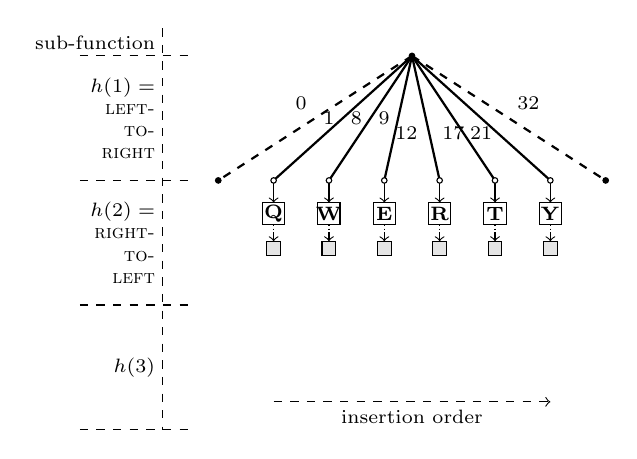
\begin{tikzpicture}[scale=1.]

\newcommand\Y{-45}
\newcommand\ADDY{-8}

  \scriptsize
  \draw[dashed] (0pt,10pt) node[anchor=north east]{sub-function} -- (0pt,3*\Y pt);
  \draw[dashed] (-30pt,0 pt) -- (10pt,0 pt);
  \draw[dashed] (-30pt,\Y pt) -- (10pt,\Y pt);
  \draw[dashed] (-30pt,2*\Y pt) -- (10pt,2*\Y pt);
  \draw[dashed] (-30pt,3*\Y pt) -- (10pt,3*\Y pt);

  \draw (0pt,0.5*\Y pt)
  node[anchor=east, align=right]{$h(1) =$\\\textsc{left-}\\\textsc{to-}\\\textsc{right}};
  \draw (0pt,1.5*\Y pt)
  node[anchor=east, align=right]{$h(2) =$\\\textsc{right-}\\\textsc{to-}\\\textsc{left}};
  \draw (0pt,2.5*\Y pt)
  node[anchor=east]{$h(3)$};

  \begin{scope}[shift={(90pt,0pt)}]
  \draw[->,dashed](-50pt,3*\Y + 10 pt) -- node[anchor=north]{insertion order}
  (50pt, 3*\Y + 10 pt);

  %% node to node
  \scriptsize
  \draw[dashed, thick] (0pt,0pt) -- node[anchor=south east]{0} (-70pt,\Y pt);
  \draw[thick] (0pt,0pt) -- node[anchor=east]{1} (-50pt,\Y pt);
  \draw[thick] (0pt,0pt) -- node[anchor=east]{8} (-30pt,\Y pt);
  \draw[thick] (0pt,0pt) -- node[anchor=east]{9} (-10pt,\Y pt);
  \draw[thick] (0pt,0pt) -- node[anchor=north east]{12} ( 10pt,\Y pt);
  \draw[thick] (0pt,0pt) -- node[anchor=north]{17} ( 30pt,\Y pt);
  \draw[thick] (0pt,0pt) -- node[anchor=north]{21} ( 50pt,\Y pt);
  \draw[dashed, thick] (0pt,0pt) -- node[anchor=south west]{32} ( 70pt,\Y pt);
  %% node to element
  \draw[->] (-50pt,\Y pt) -- (-50pt,\ADDY + \Y pt);
  \draw[->] (-30pt,\Y pt) -- (-30pt,\ADDY + \Y pt);
  \draw[->] (-10pt,\Y pt) -- (-10pt,\ADDY + \Y pt);
  \draw[->] ( 10pt,\Y pt) -- ( 10pt,\ADDY + \Y pt);
  \draw[->] ( 30pt,\Y pt) -- ( 30pt,\ADDY + \Y pt);
  \draw[->] ( 50pt,\Y pt) -- ( 50pt,\ADDY + \Y pt);

  %% element to desambiguator
  \draw[->,densely dashdotted] ( -50pt,\ADDY + \Y pt) --
  ( -50pt,2.75*\ADDY + \Y pt);
  \draw[->,densely dashdotted] ( -30pt,\ADDY + \Y pt) --
  ( -30pt,2.75*\ADDY + \Y pt);
  \draw[->,densely dashdotted] ( -10pt,\ADDY + \Y pt) --
  ( -10pt,2.75*\ADDY + \Y pt);
  \draw[->,densely dashdotted] (  10pt,\ADDY + \Y pt) --
  (  10pt,2.75*\ADDY + \Y pt);
  \draw[->,densely dashdotted] (  30pt,\ADDY + \Y pt) --
  (  30pt,2.75*\ADDY + \Y pt);
  \draw[->,densely dashdotted] (  50pt,\ADDY + \Y pt) --
  (  50pt,2.75*\ADDY + \Y pt);

  \draw[fill=black] (  0pt,  0pt) circle (1pt);
  \draw[fill=black] (-70pt,\Y pt) circle (1pt);
  \draw[fill=white] (-50pt,\Y pt) circle (1pt);
  \draw[fill=white] (-30pt,\Y pt) circle (1pt);
  \draw[fill=white] (-10pt,\Y pt) circle (1pt);
  \draw[fill=white] ( 10pt,\Y pt) circle (1pt);
  \draw[fill=white] ( 30pt,\Y pt) circle (1pt);
  \draw[fill=white] ( 50pt,\Y pt) circle (1pt);
  \draw[fill=black] ( 70pt,\Y pt) circle (1pt);

  %% elements
  \draw[fill=white](-50pt,-4 + \ADDY + \Y pt)
  node{\textbf{Q}}+(-4pt,-4pt)rectangle+(4pt,4pt) ;
  \draw[fill=white](50pt,-4 + \ADDY + \Y pt)
  node{\textbf{Y}} +(-4pt,-4pt) rectangle +(4pt,4pt) ;
  \draw[fill=white]( 10pt,-4 + \ADDY + \Y pt)
  node{\textbf{R}} +(-4pt,-4pt) rectangle +(4pt,4pt) ;
  \draw[fill=white] ( -30pt,-4 + \ADDY + \Y pt)
  node{\textbf{W}} +(-4pt,-4pt) rectangle +(4pt,4pt) ;
  \draw[fill=white] ( -10pt,-4 + \ADDY + \Y pt)
  node{\textbf{E}} +(-4pt,-4pt) rectangle +(4pt,4pt) ;
  \draw[fill=white]( 30pt,-4 + \ADDY + \Y pt)
  node{\textbf{T}} +(-4pt,-4pt) rectangle +(4pt,4pt) ;

  %% desambiguator
  \draw[fill=gray!20] (-50pt,-2.5 + 2.75 * \ADDY + \Y pt)
  +(-2.5pt,-2.5pt) rectangle +(2.5pt,2.5pt);
  \draw[fill=gray!20] (-30pt,-2.5 + 2.75 * \ADDY + \Y pt)
  +(-2.5pt,-2.5pt) rectangle +(2.5pt,2.5pt);
  \draw[fill=gray!20] (-10pt,-2.5 + 2.75 * \ADDY + \Y pt)
  +(-2.5pt,-2.5pt) rectangle +(2.5pt,2.5pt);
  \draw[fill=gray!20] ( 10pt,-2.5 + 2.75 * \ADDY + \Y pt)
  +(-2.5pt,-2.5pt) rectangle +(2.5pt,2.5pt);
  \draw[fill=gray!20] ( 30pt,-2.5 + 2.75 * \ADDY + \Y pt)
  +(-2.5pt,-2.5pt) rectangle +(2.5pt,2.5pt);
  \draw[fill=gray!20] ( 50pt,-2.5 + 2.75 * \ADDY + \Y pt)
  +(-2.5pt,-2.5pt) rectangle +(2.5pt,2.5pt);

%%%%%%%%%%%%%%%%%%%%%%%%%%%%%%%%%%%%%%%%%%%%%%%%%%%%%%%%%%%%%%%%%%%%%%

\end{scope}

\end{tikzpicture}
}
  \subfloat[Right-to-left case with \LSEQ.]
  [\label{fig:lseqtreeexampleB} Right-to-left editing behavior.]
  {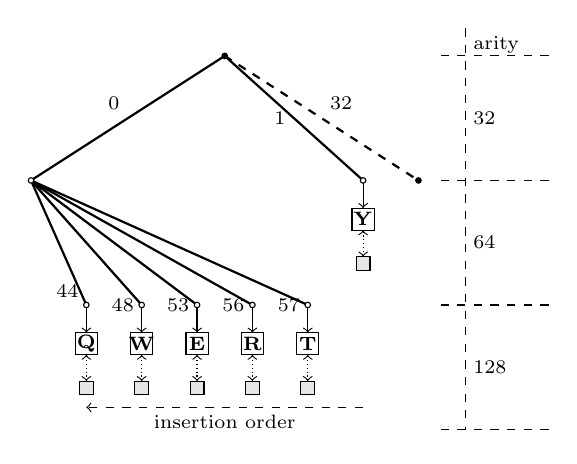
\begin{tikzpicture}[scale=1.]

\newcommand\Y{-45}
\newcommand\ADDY{-10}

  \scriptsize
  \draw[dashed] (340pt,10pt) node[anchor=north west]{arity}  -- (340pt,3*\Y pt);
  \draw[dashed] (370pt,0 pt)  --(330pt,0 pt);
  \draw[dashed] (370pt,\Y pt) -- (330pt,\Y pt);
  \draw[dashed] (370pt,2*\Y pt) -- (330pt,2*\Y pt);
  \draw[dashed] (370pt,3*\Y pt) -- (330pt,3*\Y pt);

  \draw (340pt,0.5*\Y pt)
  node[anchor=west, align=center]{$32$};
  \draw (340pt,1.5*\Y pt)
  node[anchor=west, align=center]{$64$};
  \draw (340pt,2.5*\Y pt)
  node[anchor=west, align=center]{$128$};

  \begin{scope}[shift={(93pt,0pt)}]
    \begin{scope}[shift={(160pt,0pt)}]
  \draw[->,dashed](50pt,3*\Y + 8 pt)--node[anchor=north]{insertion order}
  (-50pt,3*\Y + 8 pt);
  %% node to node
  \scriptsize
  \draw[thick] (0pt,0pt) -- node[anchor=south east]{0} (-70pt,\Y pt);
  \draw[thick] (0pt,0pt) -- node[anchor=east]{1} (50pt, \Y pt); %% Y
  \draw[thick] (-70pt, \Y pt) -- (30pt, 2 * \Y pt); %% T
  \draw[thick] (-70pt, \Y pt) -- (10pt, 2 * \Y pt); %% R
  \draw[thick] (-70pt, \Y pt) -- (-10pt, 2 * \Y pt);%% E
  \draw[thick] (-70pt, \Y pt) -- (-30pt,2 * \Y pt); %% W
  \draw[thick] (-70pt, \Y pt) -- (-50pt,2 * \Y pt); %% Q
  \draw[dashed, thick] (0pt,0pt) -- node[anchor=south west]{32} (70pt,\Y pt);

  %% node to element
  \draw[->] ( 50pt, \Y pt) -- ( 50pt, \ADDY + \Y pt); %% Y
  \draw[->] ( 30pt, 2* \Y pt) -- ( 30pt, \ADDY + 2 *\Y pt); %% T
  \draw[->] ( 10pt, 2 *\Y pt) -- ( 10pt, \ADDY + 2 *\Y pt); %% R
  \draw[->] (-10pt, 2 *\Y pt) -- (-10pt, \ADDY + 2 *\Y pt); %% E
  \draw[->] (-30pt, 2 *\Y pt) -- (-30pt, \ADDY + 2 *\Y pt); %% W
  \draw[->] (-50pt, 2 *\Y pt) -- (-50pt, \ADDY + 2 *\Y pt); %% Q

  %% element to desambiguator
  \draw[<->,densely dotted]
  ( 50pt,-8+ \ADDY + \Y pt) -- ( 50pt,2.75*\ADDY+\Y pt); %% Y
  \draw[<->,densely dotted]
  ( 30pt,-8+ \ADDY + 2* \Y pt) -- ( 30pt,2.75*\ADDY+ 2* \Y pt); %% T
  \draw[<->,densely dotted]
  ( 10pt,-8+ \ADDY + 2* \Y pt) -- ( 10pt,2.75*\ADDY+ 2* \Y pt); %% R
  \draw[<->,densely dotted]
  ( -10pt,-8+ \ADDY + 2 *\Y pt) -- (-10pt,2.75*\ADDY+ 2* \Y pt); %% E
  \draw[<->,densely dotted]
  ( -30pt,-8+ \ADDY + 2 *\Y pt) -- (-30pt,2.75*\ADDY+ 2*\Y pt); %% W
  \draw[<->,densely dotted]
  ( -50pt,-8+ \ADDY + 2* \Y pt) -- (-50pt,2.75*\ADDY+ 2*\Y pt); %% Q

  %% node
  \draw[fill=black] (0pt,0pt) circle (1pt); %% rooot
  \draw[fill=white] ( 50pt, \Y pt) circle (1pt); %% Y
  \draw[fill=white] (-70pt, \Y pt) circle (1pt); %% 0
  \draw[fill=white] ( 30 pt, 2 * \Y pt) node[anchor=east]{57} circle (1pt); %% T
  \draw[fill=white] ( 10 pt, 2 * \Y pt) node[anchor=east]{56} circle (1pt); %% R
  \draw[fill=white] (-10 pt, 2 * \Y pt) node[anchor=east]{53} circle (1pt); %% E
  \draw[fill=white] (-30 pt, 2 * \Y pt) node[anchor=east]{48} circle (1pt); %% W
  \draw[fill=white] (-50 pt, 2 * \Y pt) node[anchor=south east]{44}circle (1pt); %% Q
  \draw[fill=black] ( 70pt, \Y pt) circle (1pt);


  %% elements
  \draw[fill=white] ( 50pt, -4 + \ADDY + \Y pt)
  node{\textbf{Y}} +(-4pt,-4pt) rectangle +(4pt,4pt) ; %% Y
  \draw[fill=white] ( 30pt, -4 + \ADDY +  2 *\Y pt)
  node{\textbf{T}} +(-4pt,-4pt) rectangle +(4pt,4pt) ; %% T
  \draw[fill=white] ( 10pt, -4 + \ADDY +  2* \Y pt)
  node{\textbf{R}} +(-4pt,-4pt) rectangle +(4pt,4pt) ; %% R
  \draw[fill=white] (-10pt, -4 + \ADDY + 2 *\Y pt)
  node{\textbf{E}} +(-4pt,-4pt) rectangle +(4pt,4pt) ; %% E
  \draw[fill=white] (-30pt, -4 + \ADDY + 2 * \Y pt)
  node{\textbf{W}} +(-4pt,-4pt) rectangle +(4pt,4pt) ; %% W
  \draw[fill=white] (-50pt, -4 + \ADDY + 2 *\Y pt)
  node{\textbf{Q}} +(-4pt,-4pt) rectangle +(4pt,4pt) ; %% Q

  %% desambiguator
  \draw[fill=gray!20]( 50pt, -2.5 + 2.75 * \ADDY + \Y pt)
  +(-2.5pt,-2.5pt) rectangle +(2.5pt,2.5pt);
  \draw[fill=gray!20]( 30pt, -2.5 + 2.75 * \ADDY +2 *\Y pt)
  +(-2.5pt,-2.5pt) rectangle +(2.5pt,2.5pt);
  \draw[fill=gray!20]( 10pt, -2.5 + 2.75 * \ADDY +2*\Y pt)
  +(-2.5pt,-2.5pt) rectangle +(2.5pt,2.5pt);
  \draw[fill=gray!20](-10pt, -2.5 + 2.75 * \ADDY +2*\Y pt )
  +(-2.5pt,-2.5pt) rectangle +(2.5pt,2.5pt);
  \draw[fill=gray!20](-30pt, -2.5 + 2.75 * \ADDY +2*\Y pt)
  +(-2.5pt,-2.5pt) rectangle +(2.5pt,2.5pt);
  \draw[fill=gray!20](-50pt, -2.5 + 2.75 * \ADDY +2*\Y pt) 
  +(-2.5pt,-2.5pt) rectangle +(2.5pt,2.5pt);

\end{scope}
\end{scope}

\end{tikzpicture}
}
  \caption{\label{fig:lseqtreeexample} Example of \LSEQ's exponential trees with
    two antagonist editing behaviors to create the sequence of characters
    \texttt{QWERTY}. Contrarily to the example of
    Figure~\ref{fig:allocpathexample}, the depth of trees does not grow
    linearly.}
\end{figure}

As shown in Figure~\ref{fig:lseqtreeexample}, there exists two major differences
between \LSEQ and the state-of-the-art~\cite{preguica2009commutative,
  weiss2009logoot}:
\begin{itemize}
\item The set of possible paths in \LSEQ can be represented as an exponential
  tree~\cite{andersson1996faster,andersson2007dynamic} instead of a tree of
  constant arity. An exponential tree allows each node to have twice as many
  children as its parent. For instance, in Figure~\ref{fig:lseqtreeexample}, the
  root of the tree can have up to 32 children, each of these children can have
  up to 64 children, etc. This allows to give more space where it is required.
\item Each level of the tree has a different strategy to allocate paths. We can
  see on Figure~\ref{fig:lseqtreeexampleA} that level $h(1)$ allocates paths
  from left to right. The allocated paths increase from 1 to 21. We also see on
  Figure~\ref{fig:lseqtreeexampleB} that level $h(2)$ allocates from right to
  left. The allocated paths decrease from 57 down to 44.
  
% % Thus, paths are series of integers [$\ell_1.\ell_2\ldots\ell_e$] with, for
% % example, $\ell_1\in\mathbb{N}_{<2^5}$, then $\ell_2\in \mathbb{N}_{<2^6}$, and
% % $\ell_{e}\in\mathbb{N}_{<2^{e+4}}$.  Figure~\ref{fig:lseqtreeexample} shows
% % that
% Characters in the first level have a path between [1] and [31] while characters
% in the second level have a path between [0.1] and [31.63]. 
% Pascal: keep that for complexity analysis.
%\noindent The binary
% size of a path becomes
% $\textstyle\sum\nolimits_{i=1}^{e}\log_2{2^i}=\sum\nolimits_{i=1}^{e}i=
% {e^2-e\over{2}}$.
% For instance, in Figure~\ref{fig:lseqtreeexampleB}, the path of character
% \texttt{T} [$0.57$] requires $5 + 6 = 11$ bits.  Such quadratic growth forbids
% the existence of obvious editing behaviors leading to the worst case allocation
% as in Figure~\ref{fig:allocpathexample}.

\end{itemize}

% General idea.
If the strategy for a level suits the insertion order, then the allocation is
efficient. Otherwise, the level is sacrificed (e.g. the first level in
Figure~\ref{fig:lseqtreeexampleB}) and the next level is efficiently filled.
Thanks to the exponential growth of paths over levels, \LSEQ compensates the
sacrificed levels.  Combining an exponential tree with different allocation
strategies solves our problem statement.


% inserting \texttt{T} between the beginning of the sequence and \texttt{Y}
% implies finding a path between [0] and [1]. Since there is not enough space
% at this level, the new path  There are not enough space


% the number of available paths between [$3.1$] and [$4.0$] is 62: from [$3.2$] up
% till [$3.63$].

% Pascal: And lets go for detail explanation.
Algorithm~\ref{algo:allocpath} firstly processes the size of the new path by
progressively exploring the available paths between the adjacent paths. For
instance, in Figure~\ref{fig:lseqtreeexampleB}, the character \texttt{T} needs a
path between the paths [$0$] and [$1$]. There is not enough room for a new path
between [$0$] and [$1$], but there are $63$ available paths
%\footnote{For now, we
%  assume that there are only 10 possible values for each concatenation of the
%  path.}
between [$0.0$] and [$1.0$]. Thus, the new path will comprise 2 concatenations:
[$0.X$] where $X$ is yet to determine.

\noindent Secondly, a hash function $h$ delegates the choice of path to a
sub-allocation function. The hash function returns a result depending on the
size of the new path. For instance, in Figure~\ref{fig:lseqtreeexample}, the
sub-allocation function of paths of size 1 is \textsc{left-to-right}, the
sub-allocation function of paths of size 2 is \textsc{right-to-left}, etc. The
results of this hash function must be identical regardless of the
editor~\cite{nedelec2013concurrency}. For instance, all editors of an editing
session use the sub-allocation function \textsc{left-to-right} to choose the
paths of size 1. In addition, the choices between the sub-allocation functions
must follow a uniform distribution, for we do not know the future editing
behaviors, and we do not want to favor any.

% First, \textsc{allocPath} processes the distance between the two paths in order
% to retrieve the smallest level of the tree that contains enough room for the new
% element.

% Then, a \emph{hash function} $h$ defers the path allocation to a \emph{sub-allocation
% function} depending on the depth found for the new path. The hash function of
% every participant must give identical results~\cite{nedelec2013concurrency}.
% A hidden seed within the replicated document initializes it, for that all
% participants must make identical choices~\cite{nedelec2013concurrency}.


\noindent Thirdly, \LSEQ uses one of its two sub-allocation functions. One is
designed to handle left-to-right editing (Line~\ref{line:lefttoright}), i.e.,
repeated insertions at the right of the newest inserted element (see
Figures~\ref{fig:allocpathexampleA} and~\ref{fig:lseqtreeexampleA}); while the
other is designed to handle right-to-left editing (Line~\ref{line:righttoleft}),
i.e., repeated insertions in front of the newest inserted element (see
Figures~\ref{fig:allocpathexampleB} and~\ref{fig:lseqtreeexampleB}). To achieve
their design, they leave more available paths at the right (resp. at the left)
of the new path for the future insertions assumed at the right (resp. at the
left) of the newest element. Each sub-allocation function has 3 instructions. It
starts by processing the number of available paths between the adjacent
paths. For instance, there are $63$ available paths between [$0.0$] and
[$1.0$]. Then, it shrinks the range of allocation with a $boundary$ value. Set
to $10$, the function only considers $10$ among the $63$ available paths. Then,
depending on the design of the sub-allocation function, it chooses among the
paths in the processed range starting from one of the adjacent paths. For
instance, in Figure~\ref{fig:lseqtreeexampleB}, \textsc{left-to-right} chooses
the path of \texttt{Y} among the paths [1], [2], \ldots, [10];
\textsc{right-to-left} chooses the path of \texttt{T} among the paths [0.54]
[0.55], \ldots, [0.63].

\noindent Finally, the sub-allocation function uses \textsc{subPath} to truncate
or prolong the path in argument to reach the desired size. In
Figure~\ref{fig:lseqtreeexampleB}, when inserting \texttt{T},
\textsc{right-to-left} starts from the next path [$1$] prolonged by
\textsc{subPath} to [$1.0$] and chooses a random path among the 10 preceding
paths.  The randomness aims to leave a small gap between paths -- to handle
users' minor corrections -- even in presence of concurrent insertions. The
resulting path of \texttt{T} is $[1.0] - 7 = [0.57]$.

% There exists a major difference between \LSEQ and the
% state-of-the-art~\cite{preguica2009commutative, weiss2009logoot}: the set of
% possible paths in \LSEQ can be represented as an exponential
% tree~\cite{andersson1996faster,andersson2007dynamic} instead of a tree of
% constant arity. An exponential tree allows each node to have twice as many
% children as its parent. For instance, if the root of the tree can have up to 32
% children, each of these children can have up to 64 children, etc. Thus, the
% results of \textsc{getDepthInterval} change slightly: the paths are series of
% integers [$\ell_1.\ell_2\ldots\ell_e$] with, for example,
% $\ell_1\in\mathbb{N}_{<2^5}$, then $\ell_2\in \mathbb{N}_{<2^6}$, and
% $\ell_{e}\in\mathbb{N}_{<2^{e+4}}$. Thus, the number of available paths between
% [$3.1$] and [$4.0$] is 62: from [$3.2$] up till [$3.63$].

% \noindent The binary size of a path becomes
% $\textstyle\sum\nolimits_{i=1}^{e}\log_2{2^i}=\sum\nolimits_{i=1}^{e}i=
% {e^2-e\over{2}}$.
% For instance [$3.60$] requires $5 + 6 = 11$ bits.  Such quadratic growth forbids
% the existence of obvious editing behaviors leading to the worst case allocation
% (e.g. Figure~\ref{fig:allocpathexample}). This emphasizes the need of two
% sub-allocation functions.


% Similarly to the example of Figure~\ref{fig:allocpathexample} the example given
% in Figure~\ref{fig:lseqtreeexample} depicts the resulting trees after two
% antagonist scenarios creating the sequence \texttt{QWERTY}
% \begin{inparaenum}[(i)]
% \item the left-to-right insertions sequence [($\texttt{Q},\,0$), ($\texttt{W},\,1$),
%   \ldots] and
% \item the right-to-left insertions sequence [($\texttt{Y},\,0$),
%   ($\texttt{T},\,0$), \ldots].
% \end{inparaenum}

In Figures~\ref{fig:lseqtreeexampleA} and~\ref{fig:lseqtreeexampleB}, the
exponential tree of \LSEQ starts with a maximum arity $2^5$ and doubles it at
each level. Also, it uses the left-to-right and right-to-left sub-allocation
functions at the first and the second level of the tree respectively. Since the
first level of the tree uses the function designed for left-to-right editing,
the scenario involving the left-to-right editing sequence results in a tree of
depth 1. On the other hand -- and contrarily to the allocation function
presented in Figure~\ref{fig:allocpathexample} -- the antagonist scenario only
leads to a tree of depth 2. Indeed, \LSEQ quickly reaches a level of the tree
where the sub-allocation function is designed to handle the right-to-left
editing behavior.

%If such editing behavior
%continues, the new allocated paths will compensate the loss of the first level.


\subsection{Complexity analysis}
\label{subsec:complexity}

\begin{figure}
  \centering
  \subfloat[\LSEQ tree filled using random editing.]
  [\label{fig:randomlseq} \LSEQ tree filled using random editing]
  {
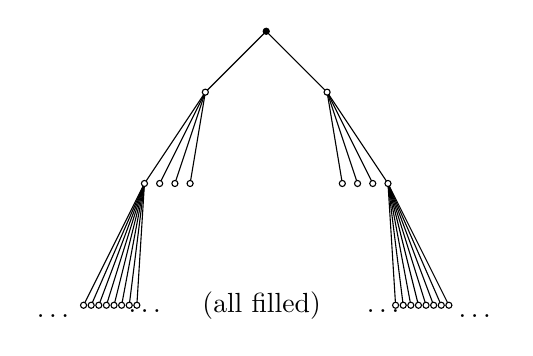
\begin{tikzpicture}[scale=1.1]

\newcommand\X{20pt}
\newcommand\Y{-20pt}

\newcommand\ADDYA{-10pt}
\newcommand\ADDYB{-30pt}

\draw (0*\X, 0*\Y) -- (-1*\X, 1*\Y);
\draw (0*\X, 0*\Y) -- ( 1*\X, 1*\Y);

\draw[fill=black] (0*\X, 0*\Y) circle (1pt); 
%% 

\draw (-1*\X, 1*\Y) -- (-1.25*\X, \ADDYA + 2*\Y);
\draw (-1*\X, 1*\Y) -- (-1.5*\X, \ADDYA + 2*\Y);
\draw (-1*\X, 1*\Y) -- (-1.75*\X, \ADDYA + 2*\Y);
\draw (-1*\X, 1*\Y) -- (-2*\X, \ADDYA + 2*\Y);
\draw (1*\X, 1*\Y) -- (1.25*\X, \ADDYA + 2*\Y);
\draw (1*\X, 1*\Y) -- (1.5*\X, \ADDYA + 2*\Y);
\draw (1*\X, 1*\Y) -- (1.75*\X, \ADDYA + 2*\Y);
\draw (1*\X, 1*\Y) -- (2*\X, \ADDYA + 2*\Y);

\draw[fill=white] (-1*\X, 1*\Y) circle (1pt); 
\draw[fill=white] (1*\X, 1*\Y) circle (1pt); 
%%

\draw(-2*\X, \ADDYA + 2*\Y) -- (-2.125*\X, \ADDYB + 3*\Y);
\draw(-2*\X, \ADDYA + 2*\Y) -- (-2.25*\X, \ADDYB + 3*\Y);
\draw(-2*\X, \ADDYA + 2*\Y) -- (-2.375*\X, \ADDYB + 3*\Y);
\draw(-2*\X, \ADDYA + 2*\Y) -- (-2.5*\X, \ADDYB + 3*\Y);
\draw(-2*\X, \ADDYA + 2*\Y) -- (-2.625*\X, \ADDYB + 3*\Y);
\draw(-2*\X, \ADDYA + 2*\Y) -- (-2.75*\X, \ADDYB + 3*\Y);
\draw(-2*\X, \ADDYA + 2*\Y) -- (-2.875*\X, \ADDYB + 3*\Y);
\draw(-2*\X, \ADDYA + 2*\Y) -- (-3*\X, \ADDYB + 3*\Y);
\draw(2*\X, \ADDYA + 2*\Y) -- (2.125*\X, \ADDYB + 3*\Y);
\draw(2*\X, \ADDYA + 2*\Y) -- (2.25*\X, \ADDYB + 3*\Y);
\draw(2*\X, \ADDYA + 2*\Y) -- (2.375*\X, \ADDYB + 3*\Y);
\draw(2*\X, \ADDYA + 2*\Y) -- (2.5*\X, \ADDYB + 3*\Y);
\draw(2*\X, \ADDYA + 2*\Y) -- (2.625*\X, \ADDYB + 3*\Y);
\draw(2*\X, \ADDYA + 2*\Y) -- (2.75*\X, \ADDYB + 3*\Y);
\draw(2*\X, \ADDYA + 2*\Y) -- (2.875*\X, \ADDYB + 3*\Y);
\draw(2*\X, \ADDYA + 2*\Y) -- (3*\X, \ADDYB + 3*\Y);

\draw[fill=white] (-1.25*\X, \ADDYA + 2*\Y) circle (1pt);
\draw[fill=white] (-1.5 *\X, \ADDYA + 2*\Y) circle (1pt);
\draw[fill=white] (-1.75*\X, \ADDYA + 2*\Y) circle (1pt);
\draw[fill=white] (-2*\X, \ADDYA + 2*\Y) circle (1pt);
\draw[fill=white] (1.25*\X, \ADDYA + 2*\Y) circle (1pt);
\draw[fill=white] (1.5 *\X, \ADDYA + 2*\Y) circle (1pt);
\draw[fill=white] (1.75*\X, \ADDYA + 2*\Y) circle (1pt);
\draw[fill=white] (2*\X, \ADDYA + 2*\Y) circle (1pt);

%%

\draw[fill=white] (-2.125*\X, \ADDYB + 3*\Y) circle (1pt);
\draw[fill=white] (-2.25*\X, \ADDYB + 3*\Y) circle (1pt);
\draw[fill=white] (-2.375*\X, \ADDYB + 3*\Y) circle (1pt);
\draw[fill=white] (-2.5*\X, \ADDYB + 3*\Y) circle (1pt);
\draw[fill=white] (-2.625*\X, \ADDYB + 3*\Y) circle (1pt);
\draw[fill=white] (-2.75*\X, \ADDYB + 3*\Y) circle (1pt);
\draw[fill=white] (-2.875*\X, \ADDYB + 3*\Y) circle (1pt);
\draw[fill=white] (-3*\X, \ADDYB + 3*\Y) node[anchor=north east]{\ldots} circle (1pt);
\draw[fill=white] (2.125*\X, \ADDYB + 3*\Y) circle (1pt);
\draw[fill=white] (2.25*\X, \ADDYB + 3*\Y) circle (1pt);
\draw[fill=white] (2.375*\X, \ADDYB + 3*\Y) circle (1pt);
\draw[fill=white] (2.5*\X, \ADDYB + 3*\Y) circle (1pt);
\draw[fill=white] (2.625*\X, \ADDYB + 3*\Y) circle (1pt);
\draw[fill=white] (2.75*\X, \ADDYB + 3*\Y) circle (1pt);
\draw[fill=white] (2.875*\X, \ADDYB + 3*\Y) circle (1pt);
\draw[fill=white] (3*\X, \ADDYB + 3*\Y) node[anchor=north west]{\ldots} circle (1pt);

\draw (0*\X, \ADDYB + 3*\Y)node{\ldots \ \ \ \ (all filled) \ \ \ \ \ldots};



\end{tikzpicture}}
  \hspace{5pt}
  \subfloat[\LSEQ tree filled using monotonic editing.]
  [\label{fig:monotoniclseq} \LSEQ tree filled using monotonic editing.]
  {
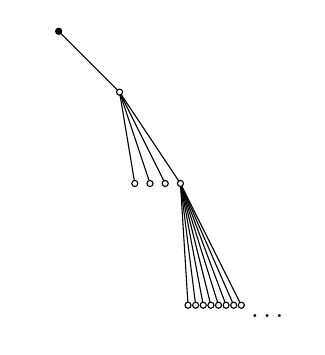
\begin{tikzpicture}[scale=1.1]

\newcommand\X{20pt}
\newcommand\Y{-20pt}

\newcommand\ADDYA{-10pt}
\newcommand\ADDYB{-30pt}

\draw (-0.5*\X, 0*\Y); %% spacing

\draw (0*\X, 0*\Y) -- ( 1*\X, 1*\Y);

\draw[fill=black] (0*\X, 0*\Y) circle (1pt); 
%% 

\draw (1*\X, 1*\Y) -- (1.25*\X, \ADDYA + 2*\Y);
\draw (1*\X, 1*\Y) -- (1.5*\X, \ADDYA + 2*\Y);
\draw (1*\X, 1*\Y) -- (1.75*\X, \ADDYA + 2*\Y);
\draw (1*\X, 1*\Y) -- (2*\X, \ADDYA + 2*\Y);

\draw[fill=white] (1*\X, 1*\Y) circle (1pt); 
%%

\draw(2*\X, \ADDYA + 2*\Y) -- (2.125*\X, \ADDYB + 3*\Y);
\draw(2*\X, \ADDYA + 2*\Y) -- (2.25*\X, \ADDYB + 3*\Y);
\draw(2*\X, \ADDYA + 2*\Y) -- (2.375*\X, \ADDYB + 3*\Y);
\draw(2*\X, \ADDYA + 2*\Y) -- (2.5*\X, \ADDYB + 3*\Y);
\draw(2*\X, \ADDYA + 2*\Y) -- (2.625*\X, \ADDYB + 3*\Y);
\draw(2*\X, \ADDYA + 2*\Y) -- (2.75*\X, \ADDYB + 3*\Y);
\draw(2*\X, \ADDYA + 2*\Y) -- (2.875*\X, \ADDYB + 3*\Y);
\draw(2*\X, \ADDYA + 2*\Y) -- (3*\X, \ADDYB + 3*\Y);


\draw[fill=white] (1.25*\X, \ADDYA + 2*\Y) circle (1pt);
\draw[fill=white] (1.5 *\X, \ADDYA + 2*\Y) circle (1pt);
\draw[fill=white] (1.75*\X, \ADDYA + 2*\Y) circle (1pt);
\draw[fill=white] (2*\X, \ADDYA + 2*\Y) circle (1pt);

%%

\draw[fill=white] (2.125*\X, \ADDYB + 3*\Y) circle (1pt);
\draw[fill=white] (2.25*\X, \ADDYB + 3*\Y) circle (1pt);
\draw[fill=white] (2.375*\X, \ADDYB + 3*\Y) circle (1pt);
\draw[fill=white] (2.5*\X, \ADDYB + 3*\Y) circle (1pt);
\draw[fill=white] (2.625*\X, \ADDYB + 3*\Y) circle (1pt);
\draw[fill=white] (2.75*\X, \ADDYB + 3*\Y) circle (1pt);
\draw[fill=white] (2.875*\X, \ADDYB + 3*\Y) circle (1pt);
\draw[fill=white] (3*\X, \ADDYB + 3*\Y) node[anchor=north west]{\ldots} circle (1pt);



\end{tikzpicture}}
  \hspace{5pt}
  \subfloat[Worst case \LSEQ tree.]
  [\label{fig:worstlseq} Worst case \LSEQ tree.]
  {
\begin{tikzpicture}[scale=1.]

\newcommand\X{20pt}
\newcommand\Y{-20pt}

\newcommand\ADDYA{-10pt}
\newcommand\ADDYB{-30pt}

%\draw (-3*\X, 0*\Y); %% spacing

\draw (0*\X, 0*\Y) -- ( 1*\X, 1*\Y);

\draw[fill=black] (0*\X, 0*\Y) circle (1pt); 
%% 

\draw (1*\X, 1*\Y) -- (2*\X, \ADDYA + 2*\Y);

\draw[fill=white] (1*\X, 1*\Y) circle (1pt); 
%%

\draw(2*\X, \ADDYA + 2*\Y) -- (3*\X, \ADDYB + 3*\Y);


\draw[fill=white] (2*\X, \ADDYA + 2*\Y) circle (1pt);

%%

\draw[fill=white] (3*\X, \ADDYB + 3*\Y) node[anchor=north west]{\ldots} circle (1pt);



\end{tikzpicture}}
  \caption{\label{fig:complexity} \LSEQ tree filled with the studied editing
    behaviors and in the worst case.}
\end{figure}


In text editing, most of the editing behaviors can be empirically summarized as
a composition of two basic editing behaviors:
\begin{itemize}
\item The random editing behavior where the author inserts new elements at what
  appears random positions in the sequence. For instance, this behavior mostly
  arises when syntactic corrections are performed, e.g. the author writes
  \texttt{QWETY} and realizes that the \texttt{R} is missing. She adds the
  missing character in a second time.
\item The monotonic editing behavior where the author repeatedly inserts new
  elements between the last inserted element and an adjacent element (after or
  before exclusively). For instance, when an author writes \texttt{QWERTY}, she
  generally starts from the first character \texttt{Q} to the last letter of the
  word \texttt{Y}. On the opposite, there exist documents mainly edited at the
  beginning
  (e.g. \url{http://en.wikipedia.org/wiki/Template_talk:Did_you_know}~\cite{nedelec2013lseq}). This
  behavior characterizes both left-to-right and right-to-left editing.
\end{itemize}

\noindent As a consequence, we focus on the space complexity analysis of \LSEQ
to random and monotonic editing behaviors. It is worth noting that monotonic
editing behavior represents an unfavorable case since it tends to unbalance the
underlying tree storing the replicated sequence. As soon as the participants
start to edit at different positions -- which is closer from a real-life use
case -- the tree becomes more balanced.
% and operations become more efficient proportionally.
The analysis does not include an average case, for it requires knowing
the average distribution of the position of edits performed by humans which is
obviously complex.

\noindent The complexity analysis also includes a worst case analysis. In the
worst case, each new identifier is bigger than the previous one. To produce such
worst case in \LSEQ, the insertions must saturate the small gap left between
identifiers (see Lines~\ref{line:plus} and~\ref{line:minus} of
Algorithm~\ref{algo:allocpath}). The editing behavior that produces such worst
case with \LSEQ is the following:
\begin{inparaenum}[(1)]
\item The user types \texttt{A} followed by \texttt{B}. The gap left between
  \texttt{A} and \texttt{B} corresponds to the $boundary$ (see
  Line~\ref{line:boundary} of Algorithm~\ref{algo:allocpath});
\item The user types $boundary$ characters between the two lastly inserted
  characters. At least the last identifier has grown;
\item Repeat the second step.
\end{inparaenum}
The editing behavior that produces such worst case with the
state-of-the-art~\cite{preguica2009commutative, weiss2009logoot} is the
following:
\begin{inparaenum}[(1)]
\item The user types a character at the beginning of the document;
\item Repeat the first step.
\end{inparaenum}


% Such editing behavior remains unlikely in collaborative editing and can be
% easily detected, for the difference between the expected growth and the actual
% growth is large.

The complexity analysis depends of the chosen structure to represent the
replica. In this section, we focus on a tree structure but other structures
(e.g. lists~\cite{weiss2009logoot}) exposing different tradeoffs could be
used. Nevertheless, the space complexity of identifiers -- the main contribution
of \LSEQ{} -- stays the same regardless of the chosen structure.



%\vspace{\PARAGRAPH}

\paragraph{Space complexity.}
%\subsubsection{Space complexity}

We distinguish the space complexity of each identifier from the space complexity
of the tree. The former is important since it directly impacts the communication
complexity, for that each identifier is broadcast to all editors; The latter is
important since it represents the replicated document stored locally by each
editor.

As stated in Section~\ref{subsec:lseqallocation}, paths
% require 1 additional bit per concatenation. In turn, paths
require $\mathcal{O}(e^2)$ bits to be encoded,
where $e$ is the depth of the element in the tree. Fortunately, the depth is
upper-bounded depending on the editing behavior that filled the exponential
tree.

The random editing behavior fills the tree at random. The repeated insertions
progressively fill the gaps in the tree without favoring any position in the
document. Over insertions, the lowest branches of the tree become filled of
elements and the depth of the tree grows slowly (see
Figure~\ref{fig:randomlseq}). Thus, the random editing behavior balances the
tree. Being exponential, the tree stores
$\textstyle\sum\nolimits_{i=1}^{k}{2^{(i^2-i)/2}}$ elements, where $k$ is the
depth of the tree. The depth of paths is upper-bounded by
$\mathcal{O}(\sqrt{\log I})$ concatenations, where $I$ is the number of
insertions. Since paths require $\mathcal{O}(e^2)$ bits to encode, paths have an
optimal logarithmic space complexity $\mathcal{O}(\log I)$. This result applies
to all variable-size identifier allocators~\cite{preguica2009commutative,
  weiss2009logoot}. A tree structure factorizes common parts of
identifiers. Overall, the space complexity is not the sum of identifiers but
$\mathcal{O}(I\log I)$.

The monotonic editing behavior fills only one branch of the tree (see
Figure~\ref{fig:monotoniclseq}). Yet, since the maximum arity grows over depths, the
growth of the tree tends decelerate over insertions. The tree stores up till
$2^{e+1}-1$ elements, where $e$ is the depth of the tree. Hence, the number of
concatenation composing a path is $\mathcal{O}(\log I)$, where $I$ is the number
of insertions. Since the binary representation of paths increases quadratically,
the space complexity of paths taken individually is upper-bounded by
$\mathcal{O}((\log I)^2)$.  Overall, the space complexity of the tree remains
upper-bounded by $\mathcal{O}(I\log I)$.

In the worst case, each insertion increases the depth of the tree. Thus, after
$I$ insertions, the tree comprises $e$ elements, where $e$ is the depth of the
tree (see Figure~\ref{fig:worstlseq}). The space complexity of paths grows
quadratically and each new allocated path contains the full tree. For instance,
the first allocated path is [$31$], the second one is [$31.63$], the third one
is [$31.63.127$], etc.  Overall, the space complexity of the tree is
$\mathcal{O}(I^2)$ too.

\begin{table}
  \vspace{\ABOVETABLES}
  \caption{\label{table:lseqspace}
    Upper bounds on space complexity of \LSEQ, Logoot and Treedoc. Where
    $I$ is the number of insertions performed on the replicated sequence.}
  \centering
  
\begin{tabularx}{0.6\textwidth}{@{}Xcc@{}}

  \toprule
  \textsc{Editing behavior} & \multicolumn{2}{c}{\textsc{Space}} \\ \cmidrule{2-3} 
                   & \textsc{Identifier} & \textsc{Sequence} \\ \midrule
  Random editing & $\mathcal{O}(\log I)$ & $\mathcal{O}(I\log I)$ \\
  Monotonic editing & $\mathcal{O}((\log I)^2)$ & $\mathcal{O}(I \log I)$ \\
  Worst case & $\mathcal{O}(I^2)$ & $\mathcal{O}(I^2)$ \\ \bottomrule
\end{tabularx}

  \vspace{-\ABOVETABLES}
\end{table}

Table~\ref{table:lseqspace} summarizes the space complexity of \LSEQ. In
particular, the expected growth of identifiers is bounded between an optimal
logarithm and a polylogarithm, hence, a sub-linear upper bound compared to the
number of insertions. To provide such improvement, \LSEQ sacrifices on its worst
case complexity that becomes quadratic. However, this worst case is made
difficult to produce, for the two sub-allocations functions with antagonist
designs settle each other's deficiency. Furthermore, if a malicious user tries
to produce the worst case, the difference in complexity makes it easy to detect,
hence, to handle. Table~\ref{table:lseqspace} also shows that compared to
state-of-the-art, \LSEQ significantly improves the identifiers size but exposes
a small overhead on the full structure, i.e. from $\mathcal{O}(I)$ to
$\mathcal{O}(I\log I)$. The tradeoff is beneficial since the communication
complexity of editors inherits from the improvement: as shown in
Algorithm~\ref{algo:crdtabstract}, each identifier is broadcast to all editors.

%\vspace{\PARAGRAPH}

\paragraph{Time complexity.}
%\subsubsection{Time complexity}
%\label{subsubsec:time}

Time complexity provides insights about the performance evolution of each
operation over insertions. They are divided between their local execution and
their remote integration.  Similarly to the space complexity, the analysis
focuses on two editing behaviors (random and monotonic) to which we add the
worst case.

The local insert operation simply consists in building a new path according to
two adjacent paths. Therefore, it depends of the depths of the latter which grow
depending on the editing behavior. Since the random editing behavior, the
monotonic editing behavior, and the worst case respectively lead to a depth
growth upper-bounded by $\mathcal{O}(\sqrt{\log I})$, $\mathcal{O}(\log I)$ and
$\mathcal{O}(I)$, the time complexity of the local part of the insert operation
follows: $\mathcal{O}(\sqrt{\log I})$, $\mathcal{O}(\log I)$ and
$\mathcal{O}(I)$.

The local delete operation simply broadcasts the identifier of the element to
remove to all participants. Hence, the time complexity is constant
$\mathcal{O}(1)$ regardless of the editing behavior.

Both the remote insert and delete operations perform the same instructions to
integrate the received result. Consequently, they have an identical time
complexity. Random, monotonic, and worst case editing behaviors respectively
lead to $\mathcal{O}(\sqrt{\log I})$, $\mathcal{O}(\log I)$ and $\mathcal{O}(I)$
levels in the exponential tree structure. Since the children of each node are
ordered by path, we perform binary searches recursively until we find the
leaf. During binary searches, the delete operation removes the nodes it explores
if they, or their children, do not contain at least another element. For
instance, considering two elements associated to the following paths: [$3.1$]
and [$3.1.2$]. If one deletes the first element, the path is kept since the path
labeled by $3$ then $1$ is still required for the second element. Then, if one
deletes the second element and the node containing it has no children, the path
and nodes are truly removed. The complexity of a binary search depends of the
level $l$ at which it is performed: $\mathcal{O}(\log 2^l)$. Repeated binary
searches lead to the upper bound
$\mathcal{O}(\textstyle\sum\nolimits_{i=1}^{e}(\log 2^i))$, where $e$ is the
depth of the tree. Replacing the depth $e$, upper bounds on time complexity are
$\mathcal{O}(\log I + \sqrt{log I})$, $\mathcal{O}((\log I)^2+\log I)$, and
$\mathcal{O}(I)$ for random, monotonic, and worst case editing behaviors
respectively. In the worst case, the algorithms perform one comparison per
element, i.e. per level, in the tree until they reach the deepest leaf.


\begin{table}
  \vspace{\ABOVETABLES}
  \caption{\label{table:lseqtime}
    Upper bounds on time complexity of \LSEQ. Where $I$ is the number of 
    insertions performed on the replicated sequence.}
  \centering
  
\begin{tabularx}{0.455\textwidth}{@{}Xcccc@{}}
  \toprule
  \textsc{Editing} & \multicolumn{4}{c}{\textsc{Time}} \\
  \textsc{behavior} & \multicolumn{2}{c}{\textsc{Local}} & \multicolumn{2}{c}{\textsc{Remote}} \\ \cmidrule(r){2-3} \cmidrule(l){4-5}
  & \textsc{ins} & \textsc{del} & \ \ \ \ \textsc{ins} & \textsc{del}  \\ \midrule
  Random & $\mathcal{O}(\sqrt{\log I})$ & $\mathcal{O}(1)$ & \multicolumn{2}{c}{$\mathcal{O}(\log I + \sqrt{\log I})$} \\
  Monotonic & $\mathcal{O}(\log I)$ & $\mathcal{O}(1)$ & \multicolumn{2}{c}{$\mathcal{O}((\log I)^2 +\log I)$} \\
  Worst case & $\mathcal{O}(I)$ & $\mathcal{O}(1)$ & \multicolumn{2}{c}{$\mathcal{O}(I)$} \\ \bottomrule
\end{tabularx}


  \vspace{-\ABOVETABLES}
\end{table}

To interface the user's view of the document with the underlying replicated
sequence, an additional lookup operation is necessary. Its goal is to retrieve
the identifier of the element at the specified index in the sequence, and
converse. Since the structure is a tree, this access is not direct.

To consistently manage the translation between sequence structure and the tree
structure, the latter stores with each node the number of elements included in
its sub-trees. Each insertion and removal updates these counters as they explore
a path. Then, processing an index comes down to count the number of elements in
the siblings of explored nodes starting from the beginning or the end of the
sequence. Unfortunately, it can be costly depending on the editing behavior that
filled the tree.

The random editing behavior leads to an exponential tree of depth bounded by
$\mathcal{O}(\sqrt{\log I})$. In such a case, a very small portion of the whole
tree will be explored. The upper bound happens when the explored nodes are
exactly in the middle of its siblings, for it forces to check at least half of
these sibling per depth. Since each node stores twice as much children as its
parents. The number of siblings to check doubles at each depth. Overall, the sum
of these siblings is equal to the number of node at the deepest level, which is
$\mathcal{O}(2^{\sqrt{\log I}})$ elements. 

From an identical reasoning, the lookup operation after monotonic editing --
which also constitutes the worst case for this operation -- is upper-bounded by
$\mathcal{O}(I)$. Indeed, only one branch is filled and explored. The counters
become useless since all nodes but one have only one child. The exploration
directly ends up in the deepest level containing $\mathcal{O}(2^{\log_2 I})$
elements where half of them must be checked leading to
$\mathcal{O}(I)$.

\begin{table}
  \vspace{\ABOVETABLES}
  \caption{\label{table:lseqlookup}
    Upper bounds on time complexity of the lookup on a \LSEQ structure.
    Where $I$ is the number of insertions performed on the replicated sequence.}
  \centering
  
\begin{tabularx}{0.6\textwidth}{@{}Xc@{}}
  \toprule
  \textsc{Editing behavior} & \textsc{Time} \\
  & \ \ \ \ \ \ \ \ \ \textsc{Look-up} \ \ \ \ \ \ \ \ \ \\ \midrule
  Random editing & $\mathcal{O}(2^{\sqrt{\log I}})$ \\
  Monotonic editing & $\mathcal{O}(I)$ \\
  Worst case & $\mathcal{O}(I)$ \\ \bottomrule
\end{tabularx}


  \vspace{-\ABOVETABLES}
\end{table}

Tables~\ref{table:lseqtime} and~\ref{table:lseqlookup} summarize the time
complexity of operations. The exponential tree structure leads to efficient
update operations. Its drawback lies in the lookup operation making the link
between the sequence and the tree. In particular, monotonic editing leads to the
worst case scenario where the access grows linearly. Fortunately,
\begin{inparaenum}[(i)]
\item the view should not be updated if the index of the change falls outside
  the user's visibility window. Thus, the lookup can stop earlier if it explores
  the tree outside the scope;
\item keeping fast accesses to the newest path and its adjacent paths removes
  the cost of the lookup, for the repeated insertions -- if monotonic -- alone
  can maintain these fast accesses up-to-date.
\end{inparaenum}

%\vspace{\PARAGRAPH}

\paragraph{Summary.}
%\subsubsection{Summary}

The complexity analysis reveals the improvements brought by \LSEQ as well as
their cost.  \LSEQ sacrifices on its worst case complexity to improve on other
editing behaviors that are considered more likely to happen in collaborative
editing. The most important result is the polylogarithmic space complexity of
identifiers, for it applies on communication complexity. In comparison,
state-of-the-art allocators~\cite{preguica2009commutative, weiss2009logoot} only
provided linearly upper-bounded identifiers. Other analysis such as the local
space consumed by the replicated structure, and the time complexity of provided
operations shows that the tree as replicated structure is
efficient. Nonetheless, based on preferences, one could choose an array -- as a
flat version of the tree -- to improve the performance of operations at the cost
of increased memory usage~\cite{weiss2009logoot}.  Section~\ref{sec:experiments}
validates our complexity analysis on experiments. The next section describes the
other components necessary to build a decentralized collaborative editor that
scales.

%%% Local Variables: 
%%% mode: latex
%%% TeX-master: "../paper"
%%% End: 